\chapter{Methods}
\label{cap:Methodology}

\section{Study Design}
For participant recruitment, newspaper articles and posters were created and published in the two study locations (Hanover and Geneva). From various responses, 72 healthy retirees were selected, with 32 from Geneva and 40 from Hanover. All participants were native or fluent in either German or French, depending on the site. The individuals were right-handed and had no more than six months of musical practice throughout their life. None of the participants relied on hearing aids. If they had any current or past neurological diseases, mild cognitive impairments, or early-stage dementia, they were excluded from the experiment. Additionally, none of the participants had any cardiovascular disease, hypertension, obesity, diabetes, or clinical depression.

\minisec{Tests}
Initially, information regarding age, sex, income, and educational level was collected, as shown in Table \ref{tab:demographic}. The income levels were defined on a scale of 1 to 5, indicating the percentage of the national average income: 1 (<25\%), 2 (25-75\%), 3 (75-125\%), 4 (125-175\%), and 5 (>175\%). Similarly, educational levels were scored from 1 to 6: 1 (elementary school), 2 (middle school), 3 (high school), 4 (bachelor's degree), 5 (master's degree), and 6 (PhD).
The participants' cognitive performance was assessed using the Cognitive Telephone Screening Instrument (CogTel). CogTel consists of six subtests that evaluate prospective memory, verbal short-term memory, working memory, verbal fluency, inductive reasoning, and verbal long-term memory. The scores range from 0 (lowest) to 60 (highest) \cite{Kliegel2007}.
Additionally, the participants completed the Cognitive Reserve Index questionnaire (CRIq) to evaluate their cognitive reserve. The CRIq calculates a score based on their educational background, working experience, and the frequency of engaging in various leisure activities such as sports, culture, and travel. An average score is derived from these factors. Scores below 70 indicate a very low cognitive reserve, while scores above 130 indicate a high cognitive reserve \cite{Nucci2012}.
%Furthermore, the participants' subjective assessment of quality of life was measured using the World Health Organization Quality of Life-BREF (WHOQOL-BREF) questionnaire \cite{WHO2012}. This questionnaire assesses four different domains: The physical domain inclues information about pain, sleep, medication use, and mobility. The psychological domain consists of statements about self-esteem, positive and negative feelings, and overall psychological well-being. The social relationships domain focuses on the participants' relationships, social support, and satisfaction with their social interactions. The environment domain assesses the participants' satisfaction with various aspects such as finances, leisure activities, home environment, and access to health services. The scores obtained from the WHOQOL-BREF questionnaire are computed and then transformed to a scale ranging from 0 to 100, with higher scores indicating a better quality of life in each domain. This assessment provides insight into the participants' subjective well-being and their perception of various life domains.

\begin{table}[h]
	\centering
	\caption{Demographic Information of the Sample}
	\label{tab:demographic}
		\renewcommand{\arraystretch}{1.2}
	\vspace{\medskipamount}
	\begin{tabular}{lcc}
		&     &  mean(SD)        \\
		\hline
		Age       &  & 69.6 (3.2) \\
		Education &  & 3.9 (1.4)  \\
		CogTel    &  & 31.0 (7.2) \\
		Income    &  & 2.9 (1.0)  \\
		Site      & Hannover         & 40 (55.6)  \\
		& Geneva         & 32 (44.4)  \\
		Sex      & Male         & 41 (56.9)  \\
		& Female         & 31 (43.1) \\
		CRIq & & 137.4 (15.1)\\
	\end{tabular}
\end{table}
To assess the participants' musical engagement ability, they were required to complete the Goldsmiths Musical Sophistication Index (Gold-MSI) self-report inventory for non-musicians \cite{Mullensiefen2014}. The Gold-MSI consists of six sub-scales that measure different facets of musical sophistication: The Active Engagement evaluates active musical engagement behaviors such as reading about music and the time and money spent on musical activities. The Perceptual Abilities are musical abilities related to perception, such as listening skills. Musical Training measures the extent of musical practice and training. Singing Abilities reflects the skills and activities related to singing. The Emotional Response to Music summarizes the participant's emotional response to music. And the General Musical Sophistication score incorporates various aspects from the other sub-scales to provide an overall measure of musical sophistication.

As Table \ref{tab:goldmsi} shows the scores of the sample is way lower than the norm data provided by the developer but didn't vary as much. The Gold-MSI questionnaire, along with the Cognitive Telephone Screening Instrument (CogTel), was repeated after the intervention.
%relevant?!
\begin{table}[h]
	\centering
	\caption{GoldMSI Scores of the Sample before the Intervention}
	\label{tab:goldmsi}
			\renewcommand{\arraystretch}{1.2}
	\vspace{\medskipamount}
	\begin{tabular}{lcc}
		&    Mean(SD)  & norm(SD)    \\
		\hline
		Active Engagement        & 29.4 (8.3) & 41.52 (10.36)\\
		Perceptual Abilities & 38.7 (9.5)& 50.2 (7.86)\\
		Musical Training    & 10.2 (3.2) &26.52(11.44)\\
		Singing Abilities     & 26.9 (6.5)  &31.67 (8.72)\\
		Emotions         & 22.2 (6.0)  & 34.66 (5.04) \\
		General Musical Sophistication            & 49.3 (12.1) & 81.58 (20.62) \\
	\end{tabular}\par
	\vspace{\medskipamount}
	\textit{The norm data is taken from the large online survey "How Musical Are You?" by BBC LabUK and decribes data from 147,633 adolscent participants \cite{Mullensiefen2013}.}
\end{table}
%Additionally, the participants' musical skills were tested using the Beat Alignment Test (BAT) and the Melodic Discrimination Test (MDT). The BAT assesses an individual's ability to understand or feel a beat and determine if it aligns with the click of a metronome. In a two-alternative-forced-choice task, participants must decide which of two presented beeps is synchronized with the beat \cite{Harrison2018}.
%The MDT evaluates the participant's ability to detect differences in different short melodies. Participants are asked to identify differences in one note among three transposed versions of the same melody \cite{Harrison2017}.
%Furthermore, the participants' scale playing on the piano was tested. They were recorded while playing the following tasks without changing hand position:
%\begin{itemize}
	%\item Slowly playing an up-and-down 5-note scale (C-D-E-F-G) at a pace of 76 beats per minute, with one note played per beat along with a metronome.
	%\item Quickly playing an up-and-down 5-note scale at the same pace, with two notes played per beat along with a metronome.
	%\item Performing the "genie test," where the same note is played five times in crescendo and four times in decrescendo, without following any specific rhythm.
%\end{itemize}
%The recordings of the scale playing were analyzed to calculate the average deviation from the metronome in seconds. A score of 0 would indicate perfect alignment between the participant's playing and the metronome.\\
The participants' motivation to contribute to the study was also assessed by collecting data on their average daily practice time at home. This information was collected at three-month intervals, specifically after three months, six months, and 12 months of the intervention. 
%In the six months after the intervention the participants were asked to note their average pratice time in a music diary.
%To evaluate the participants' recent physical activity, they completed the Physical Activity Scale for the Elderly (PASE). This questionnaire collects information about the type of activity and the duration of activity per day over the past two weeks \cite{Washburn1993}. The PASE questionnaire provides insight into the participants' levels of physical activity during the intervention period.

\begin{table}[t]
	\centering
	\caption{Timeline and Tests}
	\label{tab:time}
	\vspace{\medskipamount}
	\renewcommand{\arraystretch}{1.2}
	\begin{tabular}{lr}
		time	&   activity       \\
		\hline
		t0/0 months of intervention        & %BAT, MDT, Scale,WHOQOL-BREF\\
		\\& CogTel\\
		& GoldMSI\\
		& CRIq\\	 	
		\hline
		3 months of intervention & Ode to joy Simple\\
		& Homework\\
		\hline
		t1/6 months of intervention    		& %BAT, MDT, Scale, WHOQOL-BREF\\
		\\& Homework\\
		\hline
		t2/12 months of intervention    		& %BAT, MDT, Scale, WHOQOL-BREF\\
		\\& CogTel\\
		& GoldMSI\\
		& Ode to joy Simple \\
		& Ode to joy Normal \\
		& Homework\\
	%	\hline
	%	t3/6 months after intervention   & %BAT, MDT, Scale, WHOQOL-BREF\\
	%	\\& Music Diary \\
	\end{tabular}
\end{table}

%The participants' performance on the BAT, MDT, scale playing, WHOQOL-BREF and PASE were measured at specific time points throughout the study: once at the baseline, six months after the intervention started, 12 months after the intervention started and six months after the intervention completion (see Table \ref{tab:time}).
%These repeated measurements allowed for the evaluation of any changes or improvements in musical skills, physical activity levels, and overall cognitive functioning over the course of the intervention.

\minisec{Intervention}
After collecting the baseline data, the intervention began, consisting of one year of piano practice for the participants. The practice sessions were conducted in pairs with piano students as teachers and lasted for one hour per week. The lessons followed a pre-established curriculum (see \ref{cap:Curriculum}).
In the classroom, three Yamaha e-pianos were set up for the participants to use. Additionally, each participant was provided with a Yamaha e-piano to practice at home.
The practice sessions started with imitation and listening exercises, allowing the participants to become familiar with the piano and adopt a relaxed and correct posture. Activities such as clapping, singing, and walking in rhythm were incorporated into the sessions to enhance rhythm and musicality.
Throughout the intervention, the participants gradually learned to read sheet music. A method inspired by  "Piano Prima Vista" by Jens Schlichting (Internote GmbH Musikverlag, 2013) and the Hal Leonard Adult Piano Method was utilized to teach the participants how to read and interpret musical notation.
To reinforce learning and progress, the participants were encouraged to practice for approximately 30 minutes daily at home. They were given exercises and small pieces of music to practice, which they would then present in the following week's session.
Overall, the intervention aimed to provide structured piano practice, guided by piano students, and foster daily practice habits to enhance the participants' musical skills and enjoyment of playing the piano.

\minisec{Assessment of Piano Performance}
To assess the progress of the participants' musical abilities, recordings were made after three and twelve months of piano lessons. After three months, the participants were introduced to a simplified version of Beethoven's "Ode to Joy" (refer to \ref{cap:Ode}) and given a two-week period to familiarize themselves with it. During the recording, the participants were encouraged to play continuously without restarting and to follow the instructions provided on the sheet music, including dynamics and articulation. This recording served as an evaluation of their progress after three months of piano practice.
After twelve months of piano practice, the same version of "Ode to Joy" was recorded again to investigate the long-term effects of the piano lessons. Additionally, the participants learned a new and more challenging version of the same song, which was also recorded. Therefore, each participant had three recordings documenting their progress on the piano (see Figure \ref{fig:rater}).

The progress was evaluated by assessing changes in six variables: articulation, dynamics, rhythm, pitch, fluency, and expressivity over time in the easy version of "Ode to Joy." Possible predictors, such as age, sex, income, education, study location, CRIq score, and CogTel score, were included in the analysis to explain potential changes. The factors of the Goldsmiths Musical Sophistication Index (GoldMSI) were also taken into account. Individual explanatory models were developed for each variable to identify predictors of improvement. Furthermore, it was examined whether the predictors that indicated progress in the musical parameters of the easy version of "Ode to Joy" also predicted better results in the more challenging version of the song. The analysis aimed to identify individual explanatory models for each variable. 

Having analyzed the six musical variables, the possibility of summarizing these variables into a more concise representation of \textit{musicality} was explored. To achieve this, factor analysis was employed, a statistical technique that uncovers underlying latent factors that explain the observed correlations among the variables. By identifying one general \textit{musicality} factor, we aim to capture the essence of participants' musical abilities and provide a comprehensive understanding of how these variables converge to form a cohesive musical aptitude. The generation of a general musicality factor through factor analysis will not only enhance the interpretability of the results but also allow us to draw meaningful conclusions about the participants' overall musical potential. By unifying the six variables into one overarching factor, we can more effectively examine the influence of demographic factors, such as age, gender, and musical training, on this comprehensive measure of musicality.

%\minisec{Progress of Musical Abilities}
%The results of the scale playing, BAT, and MDT were analyzed to assess changes in participants' further musical abilities over time. Similar to the evaluation of piano playing progress, possible predictors were examined and compared to the overall progress in piano playing. By doing so, the analysis aimed to extend the understanding of progress in piano playing to gain insights into the broader development of participants' musical abilities. This analysis would provide a comprehensive understanding of how participants' musical skills evolved over the course of the intervention and help identify factors that influenced their overall musical learning experience.


\section{Evaluation of Piano Performance}
The evaluation of piano recordings was carried out by nine different raters, aged 20-30 ($M=25.78, SD = 3.23$), all with extensive experience in piano playing ($M=18.1, SD = 2.71$ years). Six of the raters held at least a bachelor's degree in music studies, while two had a degree in music education and one a master's degree in psychology. On average, the raters had taught piano for three years. 
The raters were instructed to evaluate the recordings solely based on the given musical parameters. This ensured a more objective assessment and minimized the influence of subjective preferences on the evaluation results. All raters rated the recordings in different randomized orders to reduce possible effects of inattention and dependency on their individual day form.
A scale ranging from 1 to 7 was used by the raters to evaluate six different musical aspects of the the recordings. A rating of 1 represented a very low rating, while 7 indicated a very high rating of the musical parameters. The use of a seven-point scale allowed the raters to discern and evaluate finer nuances and differences in the recordings.
The raters listened to the recordings twice. Both runs consisted of five trials consisting of about 25 excerpts of "Ode to Joy" ($\sim$ 25 min). The raters performed maximally two trials a day with ample time for recovery. The runs were completed in $\sim$ 2 weeks. During the first pass, they focused on articulation, dynamics, and rhythm. The raters assessed the correct execution of indicated articulations in the musical score, such as staccato and legato. They also discerned differences in dynamics, such as forte and piano, as well as crescendos and decrescendos. Rhythmic accuracy was evaluated based on whether the played notes occurred in the correct temporal relationship, disregarding hesitations or interruptions. In the second pass, the raters evaluated fluency, pitch accuracy, and musical expressiveness. Since the subjects were completely new to the piano, fluency was rated very good when the performer could play the piece without interruptions. Pitch accuracy assessed playing only the correct notes. Musical expressiveness was intended to reflect the quality of phrasing and interpretation of the musical piece. 
Prior to each run, raters were trained by the authors by providing them with clear scoring guidelines and examples of low, medium, and high quality musical excerpts. This enabled the raters to judge the recordings based on a common framework, which allowed for comparable scoring. To control the consistency of their ratings, the raters unknowingly evaluated 30 recordings twice. Hence, in total, each rater rated "Ode to Joy" 400 times. 




\section{Statistics}
\minisec{Ratings}
After each rater had submitted all evaluations, the results were statistically analyzed. Aligning the raters' background helped minimize potential differences in their ratings, although characteristic differences remained. These differences was balanced by using the intraclass correlation coefficient (ICC) for each rater. The ICC was initially calculated individually based on the double-rated recordings. It serves as a measure of agreement between the ratings. A correlation of 0 indicates inconsistent ratings, with significantly different evaluations of the same recordings. A correlation of 1, on the other hand, indicates complete agreement in the evaluation of the double-rated recordings. The ICC(3,1) type, according to Shrout and Fleiss \cite{Shrout1979}, was used, employing the two-way mixed effects model with a consistent relationship. The ICC was calculated by subtracting the variance between subjects from the residual variance and dividing the result by the variance between subjects. For the further analysis, the ratings of each rater were weighted by the respective ICC value per variable. 

The use of a larger number of raters with a musical background and the application of an objective rating scale contributed to the objective assessment of the musical parameters of the piano recordings. This approach allows for an informed and comparable evaluation of the musical performance of the subjects and facilitated the development and improvement of their musical abilities.

\begin{figure}[h]
	\centering
	\def \svgwidth{0.9\textwidth}
	\input{Figures/interaction.pdf_tex}
	\caption{Impacts on Musical Performance}
	\label{fig:interaction}
\end{figure}

By minimizing the process model of McPhearson and Thompson \cite{McPhearson1998} through careful disicions, the potential impact on the musical performances were reduced (see Chapter \ref{cap:Background}). This simplification helped lessen the potential impacts on musical performance. We focused on understanding the characteristics of the performance and how they interacted with specific musical or non-musical factors (see Figure \ref{fig:interaction}). This approach could provide more precise insights and enhance the analysis of piano performances.


%2.	 Factor analysis (musikalischer g-Faktor)
%3.	 Improvement over time (individual musical aspects of 1, m-g-Faktor of 2)

\minisec{Modeling Piano Performance}
The data analysis was conducted using a Bayesian mulitilevel model with the R package "brms", developed by Paul Bürkner  \cite{Burkner2017, Burkner2018}. Bayesian statistics are well-suited for accommodating hierarchical models, especially when dealing with data from multiple sources or when there are dependencies among observations. In our study, data were collected from different groups (individuals) and included repeated measures from the same individuals (each rater rated all the participants), making a hierarchical model appropriate for capturing underlying variation and improving estimation accuracy (see Figure \ref{fig:rater}). 

\begin{figure}[h]
	\centering
	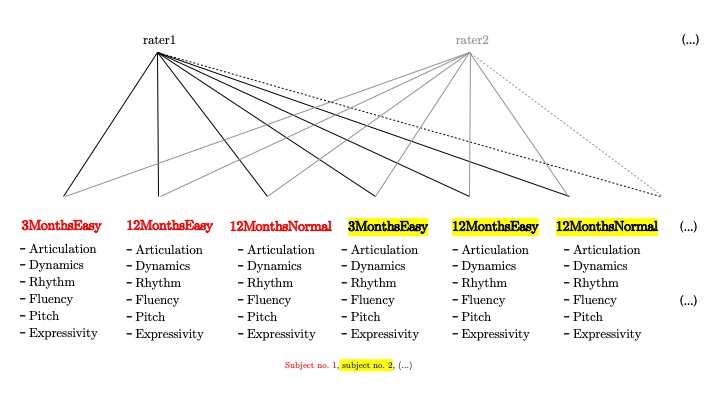
\includegraphics[width=15cm,height=10cm,keepaspectratio]{Rater}
	\caption{Rater System}
	\label{fig:rater}
\end{figure}


Bayesian apporaches have several advantages over frequentist statistics. Unlike frequentist methods that rely on statistical significance and produce dichotomous statements of significance or non-significance, Bayesian analysis provides a posterior distribution that encompasses all plausible values of the effect. Additionally, Bayesian statistics allow for the incorporation of prior knowledge or beliefs about the distribution of the data. 

To analyze results based on a scale ranging from 1 to 7, we utilized Bayesian statistics with a beta distribution, which offers a flexible and intuitive framework for modeling data within a bounded range \cite{Paolino2001}. The beta distribution is characterized by two shape parameters, $\alpha$ and $\beta$. It is well-suited for modeling proportions, probabilities, or continuous variables that are constrained within a finite range, such as a 7-point Likert scale. The versatility of the beta distribution allows it to model various response distributions, including skewed, symmetric, or bimodal distributions, making it applicable to various types of data. By specifying a prior distribution for the beta parameters ($\alpha$ and $\beta$), prior information can be included in the analysis, which can be particularly useful when limited data are available. Bayesian inference provides a framework for quantifying uncertainty in parameter estimation. By combining prior beliefs with observed data, posterior distributions can be obtained, representing a range of plausible values for the parameters. This uncertainty estimation is often valuable when interpreting results and making decisions based on the data. Within this Bayesian framework, we reported 95\% credible intervals (CI), indicating that there is a 95\% probability for the effect to fall within this range. CIs that do not include zero suggest a high likelihood that the effect is either strictly positive or negative, while CIs strongly overlapping with zero indicate a very unlikely effect. For effect sizes that only slighty overlap with zero the Probability of Direction is computed. It serves as an indicator of the existence of an effect and ranges from 50\% to 100\%. It is construed as the probality of a parameter being either strictly positive or negative . The probability of direction can be understood as a parallel to the two-sided p-value. P-values of .1, .05, .01 and .001 correspond approximately to a probability of direction of 95\%, 97.5\%, 99.5\% and 99.95\%. \cite{Makowski2019}. 

For each variable (articulation, dynamics, ryhthm, fluency, pitch, expressivitiy), a Bayesian multilevel approach was employed using the following regression equation. The data were differentiated by the Code, which represents the participants' ID, and different rater effects were considered.
\begin{equation}
	Variable \sim Demographic*time + (1 + time|Code) + (1+ time|rater)
\end{equation}
Prior to analysis, both the variables and the possible demographic predictors were centered at their means and standardized. Here, a one-unit change refers to a change of one standard deviation. Dummy variables (0|1) were used to encode sex (female|male) and site (Hanover|Geneva). Considering that the beta distribution is defined within the interval $(0,1)$, the variables were further scaled down by a  factor of seven, ensuring that the highest conceivable rating correspond to 1 and the lowest to 0. Each outcome variable was analyzed independently with respect to potential demographic predictors. 
The models allowed the slopes and intercepts of the participants to vary for a better model fit. The intercept represents the baseline performance at the beginning of the intervention, while the time effect reveals the change in performance over the study duration. 
Information about model convergence was provided by Rhat values with Rhat < 1.1 indicating satisfactory convergence. To ensure a good fit, posterior predictive checks were performed using the pp\_check function \cite{Gabry2019}.

In conclusion, the statistical apporach involved Bayesian multilevel modeling with a beta family as the response distribution. This approach offered various advantages, including the flexibility to model bounded data, incorporation of prior knowledge, and quantification of uncertainty. The individual analysis of variables allowed for a comprehensive understanding of the effects and predictors of observed changes in musical abilities. 

\minisec{Factor Analysis }
SEM 


A factor analysis was performed to uncover the complex relationships between the different musical variables.
This approach facilitated a deeper understanding of the underlying structure of musical abilities and highlighted the fundamental dimension that underlies the participants' proficiency in various musical aspects. The data used for the analysis was extracted from the calculated models, considering that the values are already weighted by the ICCs of the different raters. 
The number of latent factors was determined through scree plot analysis -- a simple line plot that displays the eigenvalues of the factors in descending order against their corresponding factor numbers. The resulting factor loadings represent the strength and direction of the relationship between the observed variables and the latent factors. Higher absolute values indicate a stronger relationship between the observed variables and the latent factors. To calculate the \textit{musicality} factor for each participant, the factor loadings ($FL_{variable}$) were multiplied by the rated values of the corresponding musical variables and then summed. The resulting composite measure represents the participant's overall \textit{musicality} score, as shown in equation \ref{eq:musicality}.
\begin{equation}
	\label{eq:musicality}
	M = (FL_A \times A) + (FL_D \times D) +\\ (FL_R\times R) + (FL_F\times F) + (FL_P \times P) + (FL_E \times E)
\end{equation}

To assess the development of the potential \textit{musicality} factor, three factor analyses were conducted. One was performed for the baseline and simple version of the "Ode to Joy" ($FA_{0,0}$),  the second after the intervention and the simple version ($FA_{1,0}$), and the third after the intervention with the more challenging version of "Ode to Joy" ($FA_{1,1}$). To avoid complicating and potentially distorting the analysis, the underlying data was extracted using models that only calculated the intercepts of each of the three measuring points. Each analysis resulted in one \textit{musicality} score for each participant at the beginning of the intervention playing the easy version of "Ode to Joy", after the intervention with the easy version, and after the intervention playing the more challenging version of "Ode to Joy". 

Subsequently, Bayesian multilevel models were established to explore potential demographic predictors. As the raters are already weighted in the input data and the input data are the estimate intercepts of all participants, the regression equation follows the simple struture shown in equation \ref{eq:musdem}:
\begin{equation}
	\label{eq:musdem}
	Musicality \sim Demographic * time
\end{equation}
Given that the data is not limited to specific values, the outcomes are modeled following a normal distribution.